\documentclass{report}
\usepackage{graphicx} % Required for inserting images
\usepackage[italian]{babel}
\usepackage{tikz}
\usepackage{hyperref}
\usepackage{amsmath}
\usepackage{xcolor}
\usepackage{float}
\usepackage{soul}
\usepackage{listings} % Per evidenziare il codice

\definecolor{lightgray}{rgb}{0.9,0.9,0.9} % Definizione colore sfondo
\definecolor{darkgreen}{rgb}{0.0, 0.5, 0.0}

\lstset{
    backgroundcolor=\color{lightgray}, % Sfondo grigio
    basicstyle=\ttfamily, % Font monospaziato
    % frame=single, % Bordo attorno al codice
    tabsize=4, % Dimensione tabulazione
    breaklines=true, % Permette di andare a capo automaticamente
    numbers = left,
    numberstyle=\small\color{gray}
}

\title{\huge\textbf{{Integrità delle Query}}}
\date{Parte II}

\begin{document}

\maketitle

\tableofcontents
\newpage

\chapter{Integrità della computazione}

Nel nostro scenario di riferimento potremo avere più \textit{data owner}; queste 
sono entità di cui ci fidiamo.

\noindent Il problema è che questi dati potrebbero essere affidati a dei \textit{cloud provider} esterni, e che possano essere soggetti a delle \textit{computazioni};
questo potrebbe essere un problema sia in termini di confidenzialità che in termini di \textbf{integrità}: 
\textit{"chi mi dice che la tua computazione sia integra?"}.

\section{Esempi}

\subsubsection{Esempio di una query}

Abbiamo l'owner che affida i propri dati ad un provider esterno;
abbiamo poi un client che effettua una query.

\begin{figure}[H]
    \centering
    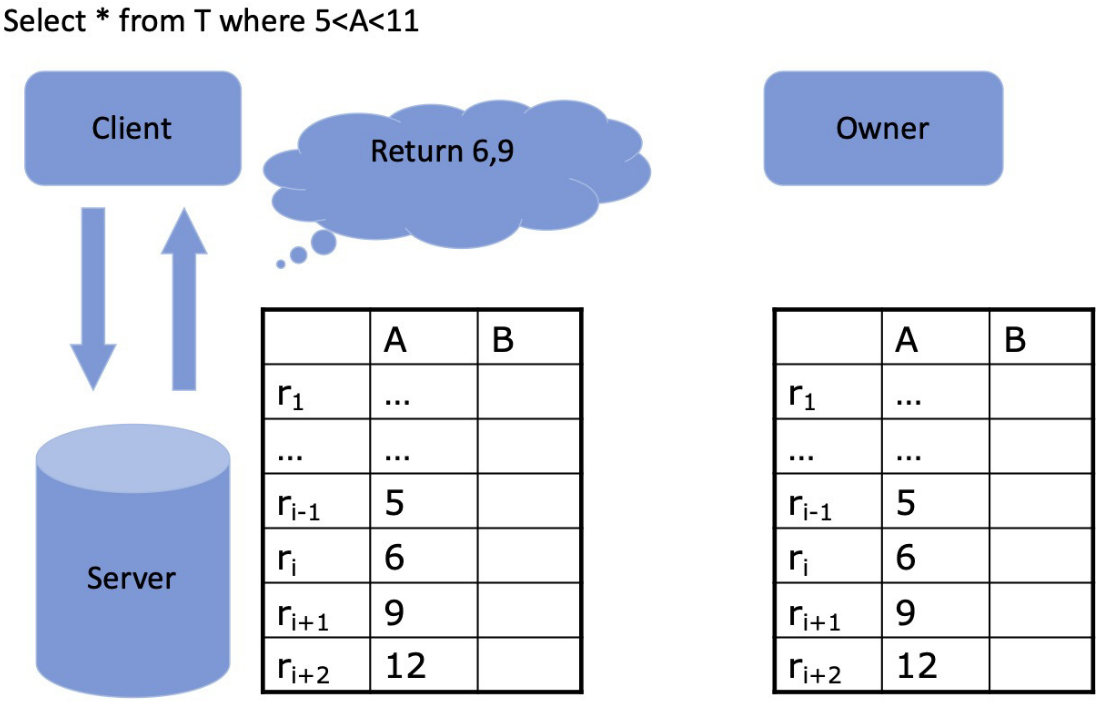
\includegraphics[width=0.7\linewidth]{images/ex1.png}
\end{figure}

\subsubsection{Esempio di query: iniezione}

Viene iniettata un'informazione fasulla; \textit{magari mi 
conviene dirti una cosa piuttosto che un'altra, le tue azioni dipendono 
da quello che ti dico\dots}

\begin{figure}[H]
    \centering
    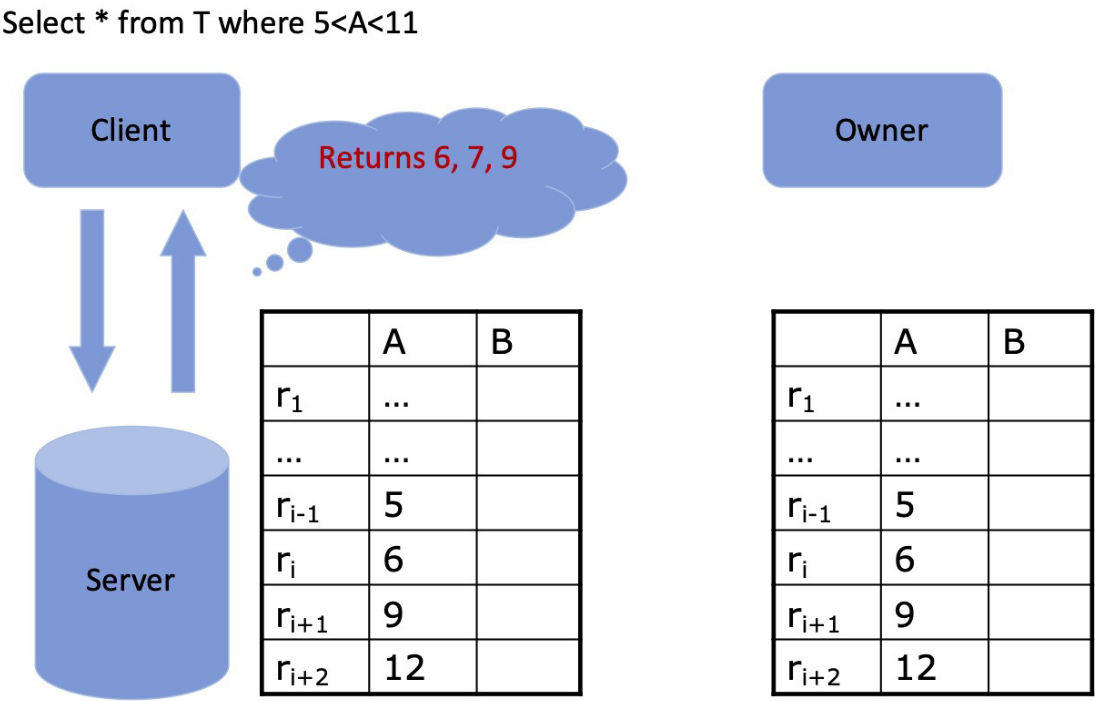
\includegraphics[width=0.9\linewidth]{images/ex2.png}
\end{figure}


\subsubsection{Esempio di query: drop}

\begin{figure}[H]
    \centering
    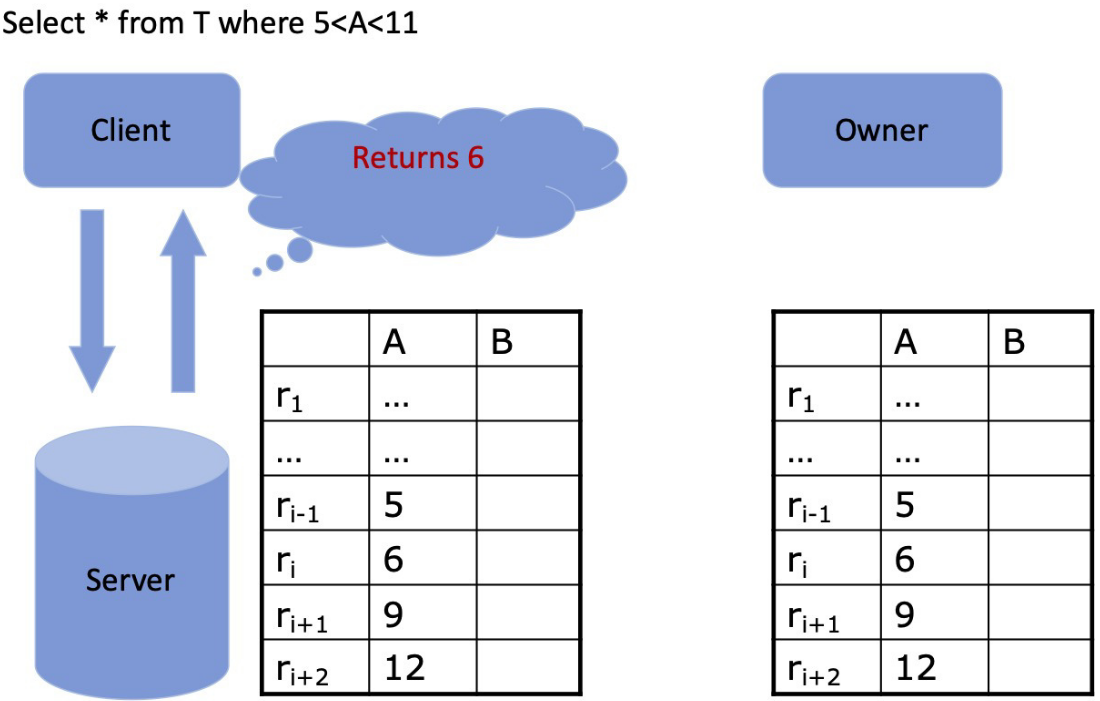
\includegraphics[width=0.9\linewidth]{images/ex3.png}
\end{figure}


\newpage
\subsubsection{Esempio di query: omissione}

I dati potrebbero essere dinamici, dunque potrebbero 
essere richieste delle operazioni di update.

\begin{figure}[H]
    \centering
    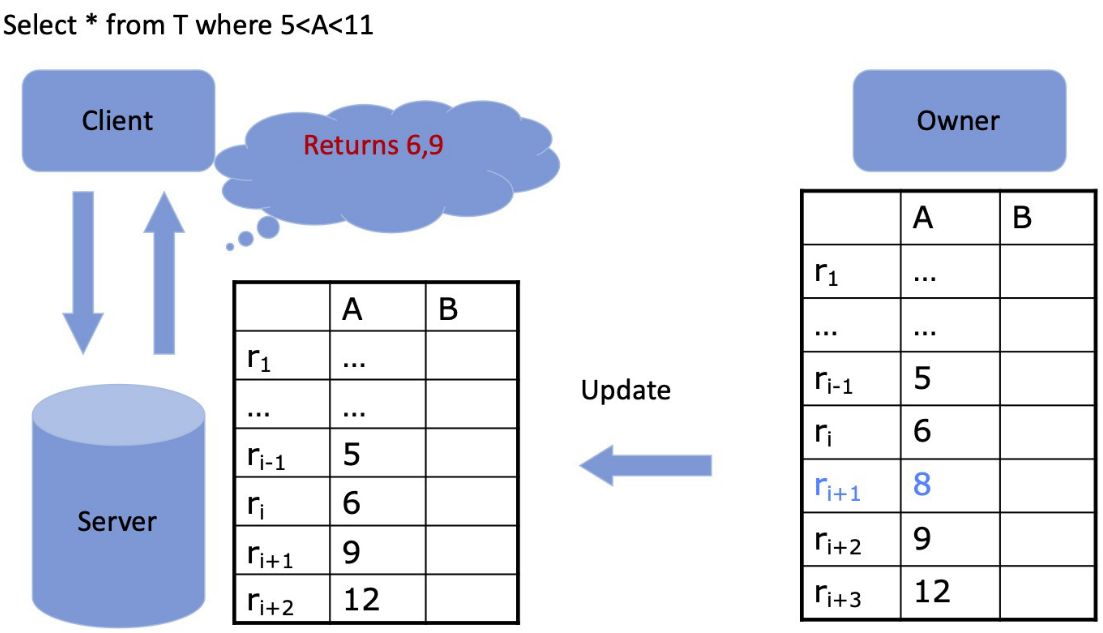
\includegraphics[width=0.9\linewidth]{images/ex4.png}
\end{figure}

\section{Integrità di storage e computazione}

Il data owner e gli utenti necessitano di meccanismi che assicurino l'integrità dei risultati 
delle query. Una query è integra se rispetta:
\begin{itemize}
    \item \textbf{Correttezza:} il risultato viene calcolato sui dati veri dell'owner (primo esempio)
    \item \textbf{Completezza:} il risultato calcolati su tutti i dati (secondo esempio)
    \item \textbf{Freschezza:} il risultato è calcolato sull'ultima versione dei dati che l'owner 
    ha dato (terzo esempio)
\end{itemize}


\noindent Ci sono due diversi tipi di approcci per rispondere al problema di integrità, 
ciascuno con i suoi vantaggi e svantaggi:
\begin{itemize}
    \item \textbf{Deterministico:} \textit{se il risultato di una computazione è integro, sono sicuro 
    al 100\% che sia integro}

    \noindent Queste tecniche vengono implementate in modo che l'owner dà al provider, oltre ai 
    dati da gestire, anche delle strutture ausiliarie che vengono sfruttate per verificare l'integrità della computazione 
    \item \textbf{Probabilistico:} \textit{ti dico sempre se è integro o no, ma non con certezza 
    assoluta ma con una certa probabilità; c'è della probabilità di fare degli errori}

    \noindent Perché si usano questi approcci? Sono tecniche che hanno lo svantaggio di non 
    avere la certezza assoluta ma che hanno altri vantaggi (che vedremo più avanti); il fatto 
    che non avere certezza sia un problema dipende da caso a caso.

    \noindent In queste tecniche il \textit{qualcosa di auisiliario} sono dei "dati finti" (marcatori)
    che "aggiungo" ai dati veri; dalla presenza o meno capisco se la query è integra o no (se prima c'erano e poi 
    non ci sono più, probabilmente c'è un errore)
\end{itemize}

\chapter{Approcci deterministici}

L'idea è che il proprietario \textit{dà fuori} i dati e una struttura 
da lui calcolata. Quando il client vuole fare una computazione, restituisce 
oltre al risultato anche un \textit{qualcosa in più} usando la struttura 
dati; questo prende il nome di 
\textbf{verification object}: è ciò che permette di verificare se il risultato della 
query è integro. 

\begin{figure}[H]
    \centering
    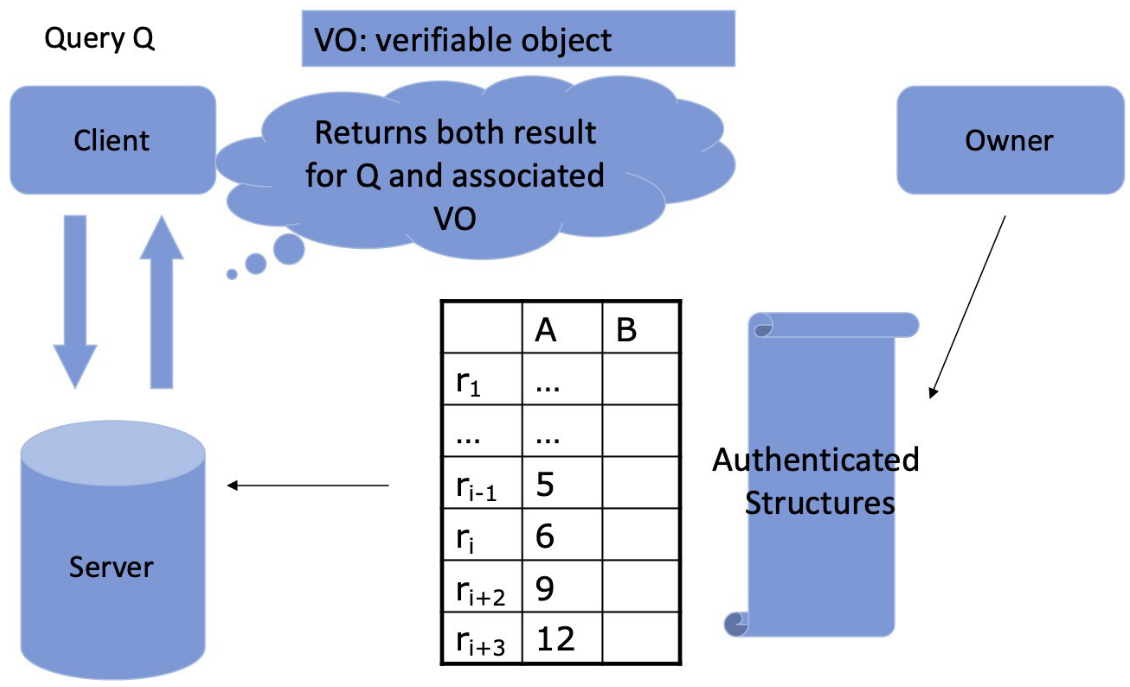
\includegraphics[width=0.8\linewidth]{images/det-idea.png}
\end{figure}






















\end{document}